\documentclass[12pt,a4paper]{article}

\usepackage{graphicx}
\usepackage[left=1.5cm,right=1.5cm,top=2cm,bottom=2cm]{geometry}
\usepackage{listings}
\usepackage{lstlang-go}
\usepackage{jslistings}
\usepackage{solidity-highlighting}
% % Copyright 2017 Sergei Tikhomirov, MIT License
% https://github.com/s-tikhomirov/solidity-latex-highlighting/

\usepackage{listings, xcolor}

\definecolor{verylightgray}{rgb}{.97,.97,.97}

\lstdefinelanguage{Solidity}{
	keywords=[1]{anonymous, assembly, assert, balance, break, call, callcode, case, catch, class, constant, continue, constructor, contract, debugger, default, delegatecall, delete, do, else, emit, event, experimental, export, external, false, finally, for, function, gas, if, implements, import, in, indexed, instanceof, interface, internal, is, length, library, log0, log1, log2, log3, log4, memory, modifier, new, payable, pragma, private, protected, public, pure, push, require, return, returns, revert, selfdestruct, send, solidity, storage, struct, suicide, super, switch, then, this, throw, transfer, true, try, typeof, using, value, view, while, with, addmod, ecrecover, keccak256, mulmod, ripemd160, sha256, sha3}, % generic keywords including crypto operations
	keywordstyle=[1]\color{blue}\bfseries,
	keywords=[2]{address, bool, byte, bytes, bytes1, bytes2, bytes3, bytes4, bytes5, bytes6, bytes7, bytes8, bytes9, bytes10, bytes11, bytes12, bytes13, bytes14, bytes15, bytes16, bytes17, bytes18, bytes19, bytes20, bytes21, bytes22, bytes23, bytes24, bytes25, bytes26, bytes27, bytes28, bytes29, bytes30, bytes31, bytes32, enum, int, int8, int16, int24, int32, int40, int48, int56, int64, int72, int80, int88, int96, int104, int112, int120, int128, int136, int144, int152, int160, int168, int176, int184, int192, int200, int208, int216, int224, int232, int240, int248, int256, mapping, string, uint, uint8, uint16, uint24, uint32, uint40, uint48, uint56, uint64, uint72, uint80, uint88, uint96, uint104, uint112, uint120, uint128, uint136, uint144, uint152, uint160, uint168, uint176, uint184, uint192, uint200, uint208, uint216, uint224, uint232, uint240, uint248, uint256, var, void, ether, finney, szabo, wei, days, hours, minutes, seconds, weeks, years},	% types; money and time units
	keywordstyle=[2]\color{teal}\bfseries,
	keywords=[3]{block, blockhash, coinbase, difficulty, gaslimit, number, timestamp, msg, data, gas, sender, sig, value, now, tx, gasprice, origin},	% environment variables
	keywordstyle=[3]\color{violet}\bfseries,
	identifierstyle=\color{black},
	sensitive=false,
	comment=[l]{//},
	morecomment=[s]{/*}{*/},
	commentstyle=\color{gray}\ttfamily,
	stringstyle=\color{red}\ttfamily,
	morestring=[b]',
	morestring=[b]"
}

\lstset{
	language=Solidity,
	backgroundcolor=\color{verylightgray},
	extendedchars=true,
	basicstyle=\footnotesize\ttfamily,
	showstringspaces=false,
	showspaces=false,
	numbers=left,
	numberstyle=\footnotesize,
	numbersep=9pt,
	tabsize=2,
	breaklines=true,
	showtabs=false,
	captionpos=b
}
\usepackage{multirow}

\setlength{\parindent}{0em}

\begin{document}

\noindent
\begin{minipage}{120mm}
        {\huge {\bf School of Informatics}}\\
        {\Large {\bf Blockchains and Distributed Ledgers}}\\

        {\Large Assignment 3}\\
        {\normalsize Erodotos Demetriou (s2187344)}
\end{minipage}
\hfill
\begin{minipage}{40mm}              
        
\includegraphics[width=40mm]{crest.png}
\end{minipage}

\begin{center}
\rule{\linewidth}{0.5mm}
\end{center}

\section*{Part 1}

For Part A of this assignment we are required to interact with a smart contract
deployed on the \emph{Ethereum Ropsten network}. In more detail, we should call
the \emph{register} method, giving as input arguments a secret key and our student
number. Since \emph{Ethereum} is a public Blockchain, everything can be accessed
on chain. Hence, the following script was used to retrive the secret key from
the smart contract's storage. \\

\begin{lstlisting}[language=JavaScript]
const Web3 = require('web3');

var web3 = new Web3(new Web3.providers.HttpProvider('https://ropsten.infura.io/v3/0ab1814012ad4231965d67bf98a40b1a'));

var contract_address = '0xde3a17573B0128da962698917B17079f2aAbebea';

web3.eth.getStorageAt(contract_address, 1).then(result => {
    console.log(web3.utils.hexToString(result));
});
\end{lstlisting} 

\vspace{5mm}

The found key is : \emph{actually...;)}. We imported the smart contract source
code and deployed address into remix and finally called the \emph{register}
function with input \emph{actually...;)} and \emph{s2187344} as inputs. \\

Transaction Hash : 0xc6ebbfea38258b115d07d5826667dfdd2445a5cbe277f0c3e18fa5a294ef3d32

\section*{Part 2 A}

\subsection*{Smart Contract High-Level Description}

Part 2 A of this assignment regards implementing and deploying a custom token.
Its requirements include allowing users to exchange ETH for tokens, sell their
tokens back for ETH, and transfer tokens between accounts. Also, the users can
view their balance by calling the smart contract. Besides that, the token owner
can change the token's price if there is enough balance in the smart contract. \\

To achieve that, we introduced the concept of liquidity providers. Liquidity
providers are individuals willing to deposit their ETH to the smart contract and
receive tokens as rewards whenever a new buyer purchases the token in the
future. Next, we provide a real-world example of using this mechanism to
understand its functionality better. \\

\begin{figure}[htpb]
    \begin{center}
        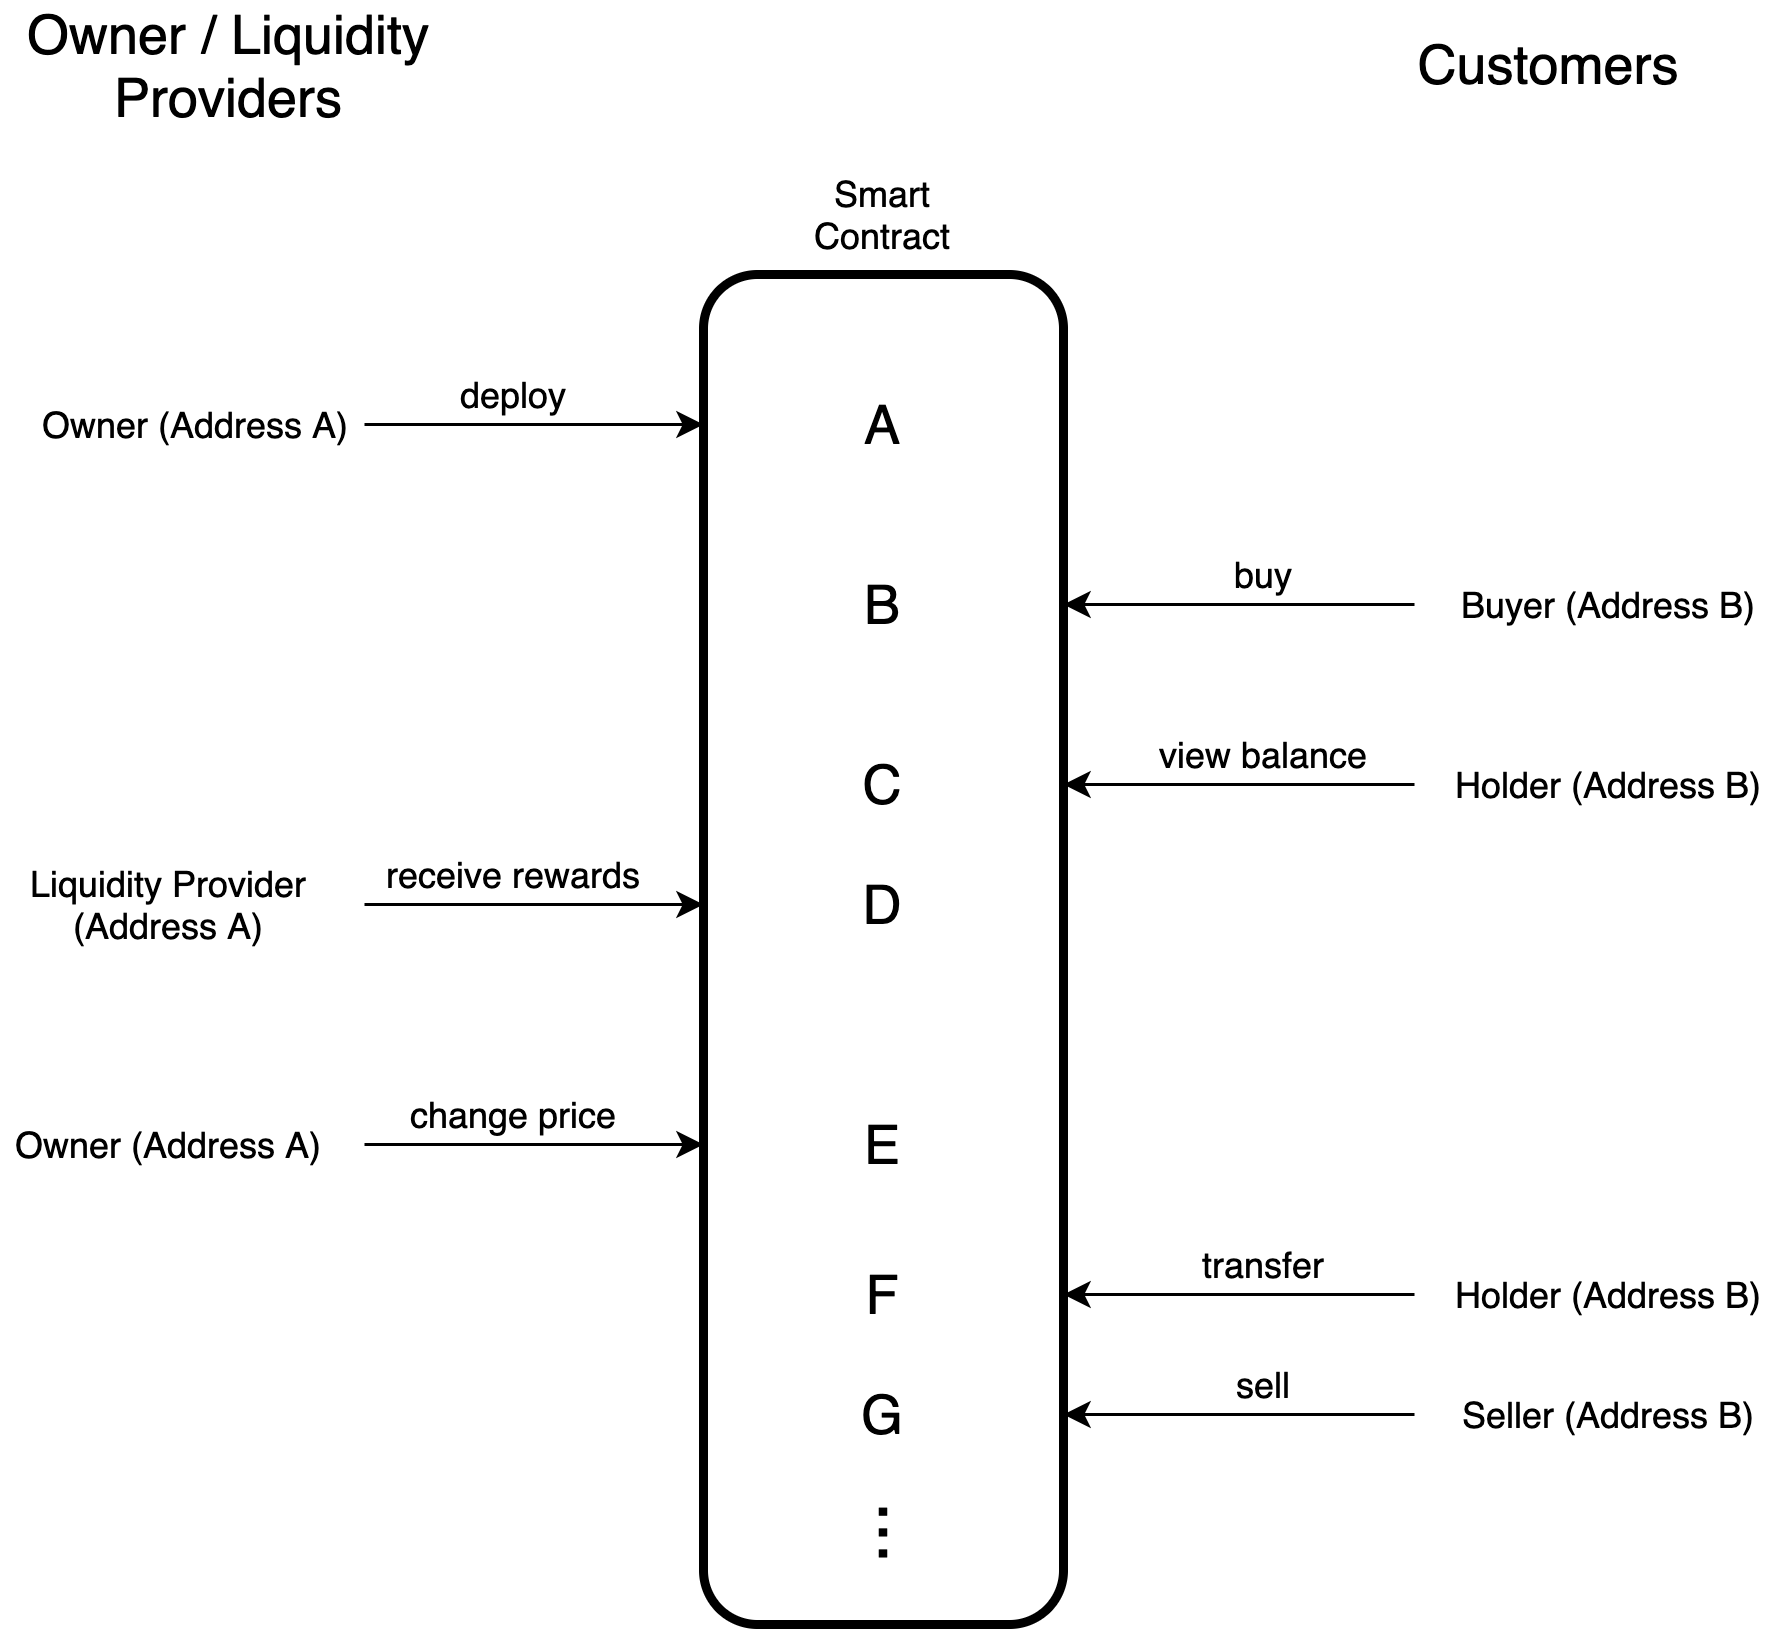
\includegraphics[height=8cm]{execution_flow.png}
        \caption{Smart Contract Execution Workflow Example}
        \label{fig:smart-contract-example}
    \end{center}
\end{figure} 

Figure \ref{fig:smart-contract-example} illustrates the smart contract's life cycle. In
step A, the owner (address A) deploys the smart contract providing 100 Wei. This
automatically registers him as the first liquidity provider. Next, in step B, we
can observe a buyer (address B) conducting a buy request to the smart contract.
For instance, he wants to buy 30 tokens priced at ten Wei each. Hence, he has to
send 300 Wei to the smart contract and provide the number of tokens as an input
parameter. We check for the validity of the input data, and if everything is
accurate, we proceed. 10\% of the purchased tokens is contributed into a rewards
pool while the customer receives 90\%. We have to mention that for simplicity
objectives in calculating the percentage, we allow purchases of multiples of 10.
Later, in step C the buyer can view its balance by calling the getBalance()
method of the smart contract. At this point (D), a liquidity provider can
receive rewards from the rewards pool. He will get a portion of tokens according
to the fraction of liquidity he provided to the total liquidity. In other words,
each provider can increase the rewards he receives by offering more liquidity.
\\

Nonetheless, we have to note that because solidity does not support floats, we
restrict the amount a liquidity provider can offer to multiples of 100 Wei.
Further, if there is only one token in the rewards pool and two liquidity
providers own 50\% of it each, the smart contract will not allow them to receive
rewards because of an impossible division of 1/2. They can receive their rewards
later when the pool balance allows a fair distribution. \\

Now, suppose we want to change the price of our token. The owner can allow this
action in step E. The only constrain of this transaction is that the contract's
balance should be greater or equal to the product of circulating tokens and the
new price. \\

Moreover, a token holder can transfer its tokens to another address. This is
depicted in step F, where the user calls the smart contract providing the
receiver's address and the transfer amount of tokens. \\

Finally, any token holder may sell his tokens to the smart contract for ETH
considering the current token price in Wei. The sell token function does not
directly transfer ETH to the user. Instead, a custom library deployed on the
Ropsten network is used. One of the main challenges of this assignment was to
link an already deployed library into our smart contract. This was impossible to
achieve through remix online editor. Thus we used Truffle smart contract
development framework to achieve the desired outcome. Practically, we compiled
the customLib.sol locally to generate a reference ABI and afterward import the
library into our Token.sol contract. Since we needed to use an already deployed
instance of the library, we specified its address in the migrations javascript
file and used the link method to reference it. There follows the deployment and
link script for the operation as mentioned earlier and a detailed of smart
contract's variables, functions and events. \\

\begin{lstlisting}[language=JavaScript]
const Token = artifacts.require("Token");
const CustomLibrary = artifacts.require("customLib");

module.exports = function(deployer, accounts) {
    CustomLibrary.address = "0xc0b843678E1E73c090De725Ee1Af6a9F728E2C47"
    deployer.link(CustomLibrary, Token);
    deployer.deploy(Token, { value: "100" })
};
\end{lstlisting}

\textbf{\underline{Variables}} \\

\textbf{\emph{address owner:}} This variable is set on deployment, and stores the smart
contract's owner address.\\
\textbf{\emph{uint256 contractBalance:}} This variable stores the number of \emph{wei} deposited
into the smart contract.\\
\textbf{\emph{uint256 circulatingTokens:}}  This variable stores the number of
circulating tokens.\\
\textbf{\emph{mapping balances:}} This is a mapping variable maintaining a one to one
correspondance between a user address and the number of tokens it holds. \\
\textbf{\emph{mapping liquidityProviders:}} This is a mapping variable maintaining a one
to one correspondance between a liquidity provider user address and the amount
of liquidity it provided in \emph{wei}. \\
\textbf{\emph{uint256 numberOfProviders:}} This variable holds the number of total
liquidity providers.\\
\textbf{\emph{uint256 totalLiquidity:}} This variable holds the amount of total liquidity
provided during the complete life cycle of the smart contract.\\
\textbf{\emph{uint256 rewardsPool:}} This variable stores the amount of tokens that will
be available to liquidity providers as rewards for their services.\\
\textbf{\emph{uint256 tokenPrice:}} This variable stores the current token price in
\emph{wei}.\\

\textbf{\underline{Events}} \\

\textbf{\emph{event Purchase:}} Whenever a token purchase is fulfilled, an event stating
the buyer's address and the purchased amount, is emitted.\\
\textbf{\emph{event Sell:}} Whenever a token holder sells its tokens back to the smart
contract, a sell event is emitted. This event states the seller address and the
amount of tokens sold.\\
\textbf{\emph{event Transfer:}} Whenever a token holder transfers its tokens to an other
address a transfer event is emitted. This event states the sender and receiver
adddresses, as well as the transfered amount of tokens.\\
\textbf{\emph{event Price:}} This event is emitted whenever the smart contract owner
changes the token price.\\

\textbf{\underline{Functions}} \\

\textbf{\emph{constructor():}} This is the smart contract constractor. It is called
whenever the code is deployed for the first time, and sets the contract owner,
as the initiator of the transaction. The smart contract constructor requirement
is that the owner provides 100 \emph{wei} as initial liquidity. Thus he becomes
the first liquidity provider.\\
\textbf{\emph{buyToken():}} Whenever a buyer wants to exchange his ETH for our token has
to call this function. In more detail, he needs to provide as input the number
of tokens that he desires to purchase and send the proportional amount of ETH,
considering the token price which is in \emph{wei}.\\
\textbf{\emph{transfer():}} This function can be called by a token holder that desires to
transfer a specific amount of tokens to an other address.\\
\textbf{\emph{sellToken():}} This function enables a token holder to exchange his tokens
with ETH. He can provide the number of tokens he wants to exchange and
subsequentyl he will receive the according value of ETH considering the current
token price.\\
\textbf{\emph{changePrice():}} This function can be called only by the smart contract
owner, to change the token price. Its execution will only succed if there is
enough liquidity to pay token holders if they decide to sell their token
simultaneously.\\
\textbf{\emph{getBalance():}} This function returns the balance of tokens that are in the
posetion of the fucntion's caller.\\
\textbf{\emph{provideLiquidity():}} This is an internal function that can be triggered
through the fallback function. It receives an address and the amount of provided
liquidity. Subsequentyl, it registers this user as a liquidity provider. \\
\textbf{\emph{getReward():}} This is an internal function that can be trigered through
the fallback function and only if the caller is a registered liquidity provider.
Its execution results into receiving a proportion of the reward tokens from the
reward pool.\\
\textbf{\emph{fallback():}} This function can be used with different arguments and can
serve different purposes. If it is called providing some ETH, registers you as a
liquidity provider; Else, it can be used by liquidity provider to receive its
rewards.

\subsection*{Gas Costs Evaluation}
This section measures and evaluates the gas cost we expect to have when deploying and
interacting with the Smart Contract. \\

Gas costs appear in the following table. The Smart Contract owner has to pay
1,389,915 gas units to deploy the code. This is a high amount of gas, making the
smart contract expensive to deploy initially. \\

\begin{table}[htpb]
    \begin{center}
        \begin{tabular}{cc}
        \multicolumn{2}{c}{\textbf{Gas Costs}}                                                                \\
        \multicolumn{1}{l}{}                                                & \multicolumn{1}{l}{}            \\ \hline
        \multicolumn{2}{|c|}{\textit{\textbf{Contract Owner Fees}}}                                           \\ \hline
        \multicolumn{1}{|c|}{Contract Deployment}                           & \multicolumn{1}{c|}{1,389,915}  \\ \hline
        \multicolumn{1}{l}{}                                                & \multicolumn{1}{l}{}            \\ \hline
        \multicolumn{2}{|c|}{\textit{\textbf{Customer Fees}}}                                                 \\ \hline
        \multicolumn{1}{|c|}{buyToken()}                                   & \multicolumn{1}{c|}{65,102}   \\ \hline
        \multicolumn{1}{|c|}{sellToken()}                                  & \multicolumn{1}{c|}{62,875}   \\ \hline
        \multicolumn{1}{|c|}{transfer()}                                   & \multicolumn{1}{c|}{52,328}   \\ \hline
        \multicolumn{1}{|c|}{changePrice()}                                & \multicolumn{1}{c|}{34,639}   \\ \hline
        \multicolumn{1}{|c|}{getBalance()}                                 & \multicolumn{1}{c|}{None}   \\ \hline
        \multicolumn{1}{l}{}                                               & \multicolumn{1}{l}{}             \\ \hline
        \multicolumn{2}{|c|}{\textit{\textbf{Liquidity Provider Fees}}}                                       \\ \hline   
        \multicolumn{1}{|c|}{provideLiquidity()}                           & \multicolumn{1}{c|}{42,083}   \\ \hline
        \multicolumn{1}{|c|}{getReward()}                                  & \multicolumn{1}{c|}{35,110}   \\ \hline
        \end{tabular}
    \end{center}
\end{table}

Regarding the smart contract customers interactions, the fees are much lower.
Namely, when buying some tokens, the gas required is 65,102, while the
invocation of sellToken function costs 62,875. We can observe that buying and
selling tokens from and to the contract yields approximately the same overhead.
Next, if a token holder transfers its tokens to another address, he can use only
52,328 gas units, which is relatively cheap. Retrieving the available balance of
tokens for a specific address occurs at no expense. \\

Besides customer invocations, we have liquidity providers interacting with the
smart contract. Providing liquidity costs 42,083 gas units. When designing the
provide liquidity functionality, our goal was to keep it as cheap as possible to
motive liquidity providers to back the token sale. We can argue that this has
partially been achieved since depositing funds is cheaper than buying or selling
tokens. Furthermore, when a liquidity provider requests its rewards, the costs
are even cheaper at 35,110 gas units. Nonetheless, a liquidity provider will
amortize its investment with more profits since 10\% of each token purchase goes
to him. 

\subsection*{Potential Hazards and Vulnerablities}

Developing a Smart Contract can always be challenging. This is because, on a public-permissionless blockchains, everything is observable by everyone. This fact makes it difficult when it comes to securing users’ data. Besides that, a developer has to be alert to write code that is attack-resistant. Smart Contracts expose a broad spectrum of vulnerabilities, enabling an adversarial entity to exploit them for his interest.\\

When developing the Matching Pennies game, we took into consideration possible attacks.
The following list presents vulnerabilities and mechanisms to moderate them. \\

\textbf{\emph{DoS(Denial of Service) - Griefing: }}An attacker attempts to make a Smart Contract get stuck when executed. In the case of our implementation, a player might grieve and stop playing to halt the Smart Contract or make his opponent lose money. This is not wanted since the other player’s ETH will get stuck, and no one else will be able to play the game. \\

\textbf{\emph{Mitigation: }}To counter this type of attack, we implemented a
time limit mechanism. When a player interacts with the Smart Contract, a timer
is initiated. The other player has only 10 minutes to play his move. If the time
limit expires, the last player can request a refund and cancel the game. The
funds of the lapsed player will be kept as punishment. If a single player tries
to halt the program (i.e., only one player joins the game and his opponent
refuse), the Smart Contract owner can join, to force the first player to play.
If the first player denies playing, he will lose his money since the contract
owner can request a refund, which will reset the game. Using this technique, the
Smart Contract can never halt.\\

\textbf{\emph{Re-Entrancy: }}An attacker might try to take advantage of the
Smart Contract withdraw function by executing a re-entrancy attack. In more
detail, when he invokes a withdrawal transaction, he can drive his transaction
to a malicious fallback function on another Smart Contract that can recursively
call again and again the withdraw function, trying to get more ETH.\\

\textbf{\emph{Mitigation: }}In order to avoid such unpleasant attacks, we
execute the code of the Smart Contract in a particular way. When there is a
withdrawal invocation, we check some constraints to ensure that the transaction
sender is allowed to withdraw ETH. After that, we will pass any updates to the
state of the Smart Contract and eventually make the call that sends the
requested ETH to the recipient. It is important to make the ETH transfer after
changing the Smart Contract state. If a reentrancy attack occurs on the next
transaction, it will be stopped because function constraints will evaluate the
transaction according to the updated state.\\

\textbf{\emph{Front-Running: }}This attack happens on the Miner level. An
attacker might clone your transaction and put a much higher gas limit on it.
This results in the inclusion of his transaction to the next block instead of
yours. This is inconvenient since another player might steal your spot in the
game. \\

\textbf{\emph{Mitigation: }}There is no straightforward solution since the
problem lies at the transaction mining level. For the Matching Pennies game,
front-running will not have a significant effect, except that a player might
steal the position of another one. The disfavored player will have the
opportunity to play in another moment. \\

\textbf{\emph{Overflow/Underflow: }}Matching Pennies game does not face this
problem since it does not receive any integer value from the transaction sender.
\\

\textbf{\emph{Randomness Source Exposure: }}Matching Pennies game does not face
this problem since it does not use any random value during the code execution.
\\

\textbf{\emph{Delegation: }}Matching Pennies game does not face this problem
since it does not use code from other Smart Contracts or Libraries. \\

\textbf{\emph{\underline{Other good practices:}}} \\ 

\begin{itemize}
    \item Use \emph{call()} instead of \emph{transfer()} or \emph{send()}. Using
    \emph{call()}  might be insecure, but \emph{transfer()} and \emph{send()}
    can forward only 2300 gas. In the future gas costs might change, and 2300
    gas might not be enough. As a result using \emph{call()} properly is the
    right approach. Below we can see an example of using \emph{call()} function
    and handling its outcome correctly.\\
    \begin{lstlisting}[language=Solidity]
        (bool success, ) = msg.sender.call.value(amount)(""); 
        require(success, "Transfer failed.");
    \end{lstlisting}
    \item If you need to have a callback function, keep it simple.
    \item Any public-permissionless blockchain reveals transaction details to 
    the ledger. Due to this fact, in data-sensitive applications such as the
    Matching Pennies game, we need to hide users' data. We can do this by following a
    two-phase process: committing a value obscured by hashing the bet and some salt
    and then exposing the real value.
\end{itemize}

\subsection*{Smart Contract Deployment and Execution History}

Owner Address: 0x1959f7433D617977e144cC3Bb722D794384D562B

\begin{itemize}
    \item \textbf{Smart Contract deployment}\\
    TX Hash: 0x5ba0d9a48485c1400f72bf2d0482b869f44935ceb38cbb8a720a5d66c391ece0 \\
    Contract Address: 0x8252e289f6ef096CCb0647322102ac5459D1Df49
    \item \textbf{Buy Tokens}\\
    TX Hash: 0xeaf2f20e09dc42dbf743d6edd7618e831f3ce195967ccb4624b4b6dfa395ab88
    \item \textbf{Get Rewards}\\
    TX Hash: 0x7aef6df0c8b4a3d8f7685c3e7cc2f33117addeea284d0fd940abbab9e17c60b7
    \item \textbf{Change Price}\\
    TX Hash: 0xae26b213a00cd543b3a57e97d9f0626b18812df69fb10cc843432302442f122a
    \item \textbf{Transfer Tokens}\\
    TX Hash: 0xfa2a9b619d58b934957503f8afdd08ceafcd71e228d7d27fc357c8ad4b3c1976
    \item \textbf{Sell Token}\\
    TX Hash: 0x53be3484f8fe51bd58bc5f4aec9f0ae45711b7b8924c23f70f512ba21f0c5aa1
    \item \textbf{Provide Liquidity}\\
    TX Hash: 0x43f228412eb74dc55e40c95f5f020e4efe3bdc4b6eef91dda21a2041f08dd002\\
\end{itemize}

\subsection*{Implementation Code}
\begin{lstlisting}
// SPDX-License-Identifier: MIT
pragma solidity >=0.8.00 <0.9.0;

import "./customLib.sol";

contract Token {
    address private owner;
    uint256 private contractBalance = 0;
    uint256 private circulatingTokens = 0;

    mapping(address => uint256) private balances;
    mapping(address => uint256) private liquidityProviders;
    uint256 private numberOfProviders = 0;
    uint256 private totalLiquidity = 0;
    uint256 private rewardsPool = 0;

    uint256 public tokenPrice = 10;

    event Purchase(address indexed buyer, uint256 amount);
    event Sell(address indexed seller, uint256 amount);
    event Price(uint256 price);
    event Transfer(
        address indexed sender,
        address indexed receiver,
        uint256 amount
    );

    constructor() payable {
        require(
            msg.value == 100,
            "As the contract owner you are required to provide 100 wei liquidity"
        );
        owner = msg.sender;
        provideLiquidity(owner, msg.value);
    }

    function buyToken(uint256 amount) public payable returns (bool) {
        require(
            msg.value == amount * tokenPrice,
            "Your funds are not sufficient"
        );
        require(
            amount % 10 == 0,
            "The purchased quantity should be multiple of 10!"
        );
        circulatingTokens += amount;
        contractBalance += amount * tokenPrice;
        balances[msg.sender] += (amount * 90) / 100;
        rewardsPool += (amount * 10) / 100;
        emit Purchase(msg.sender, amount);
        return true;
    }

    function transfer(address recipient, uint256 amount) public returns (bool) {
        require(balances[msg.sender] >= amount, "Not enough balance");
        balances[msg.sender] -= amount;
        balances[recipient] += amount;
        emit Transfer(msg.sender, recipient, amount);
        return true;
    }

    function sellToken(uint256 amount) public returns (bool) {
        require(amount >= 1, "Provide positive amount of tokens!");
        require(amount <= balances[msg.sender], "Not enough balance!s");
        require(amount > 0, "Not enough balance!");
        circulatingTokens -= amount;
        balances[msg.sender] -= amount;
        contractBalance -= amount * tokenPrice;
        bool success = customLib.customSend(amount * tokenPrice, msg.sender);
        require(success, "Transfer failed!");
        emit Sell(msg.sender, amount);
        return true;
    }

    function changePrice(uint256 price) public returns (bool) {
        require(
            msg.sender == owner,
            "This function is restricted to the contract's owner"
        );
        require(
            contractBalance >= circulatingTokens * price,
            "Not enough liquidity"
        );

        tokenPrice = price;
        emit Price(price);
        return true;
    }

    function getBalance() public view returns (uint256) {
        return balances[msg.sender];
    }

    function provideLiquidity(address provider, uint256 amount) internal {
        liquidityProviders[provider] += amount;
        totalLiquidity += amount;
        contractBalance += amount;
        numberOfProviders += 1;
    }

    function getReward() internal {
        require(
            liquidityProviders[msg.sender] >= 100,
            "You are not a liquidity provider"
        );

        require(
            rewardsPool % numberOfProviders == 0,
            "You can not receive rewards now (unfair division)"
        );

        uint256 allowance = (liquidityProviders[msg.sender] / totalLiquidity) *
            100;
        balances[msg.sender] += (rewardsPool * allowance) / 100;
        rewardsPool -= (rewardsPool * allowance) / 100;
    }

    fallback() external payable {
        if (msg.value > 0) {
            provideLiquidity(msg.sender, msg.value);
        } else {
            getReward();
        }
    }
}
\end{lstlisting}

\section*{Part 2 B}

\end{document}